%!TEX root = ../template.tex
%%%%%%%%%%%%%%%%%%%%%%%%%%%%%%%%%%%%%%%%%%%%%%%%%%%%%%%%%%%%%%%%%%%%
%% chapter4.tex
%% NOVA thesis document file
%%
%% Chapter with lots of dummy text
%%%%%%%%%%%%%%%%%%%%%%%%%%%%%%%%%%%%%%%%%%%%%%%%%%%%%%%%%%%%%%%%%%%%

\typeout{NT FILE chapter4.tex}%

\chapter{Heuristic and Metaheuristic Algorithms}\label{chapt:4}
\section{Heuristic Approaches}

Heuristic approaches to solving problems such as the \Gls{TSP} are strategies designed to find sufficiently good solutions within a reasonable time, especially when an exact solution is not feasible due to the complexity \cite{Johnson2002} of the problem. These methods are essential in cases where the computational cost of finding the optimal solution is prohibitive, as is common with NP-hard problems such as the \Gls{TSP} \cite{Cormen2009}.

\subsection{Concept and Necessity}
The concept of heuristic approaches is based on the idea of making educated guesses or following intuitive algorithms that aim to find solutions that are close to the best possible, without necessarily guaranteeing optimality \cite{Papadimitriou1998}. Heuristics are characterized by their empirical strategies that make them significantly faster than exact methods in practice, albeit at the cost of potentially missing the optimal solution.

The necessity of heuristics stems from the computational intractability of many real-world problems \cite{Lawler1985}. Heuristics offer a pragmatic alternative by providing solutions that, while not guaranteed to be optimal, are sufficiently accurate for practical purposes and can be obtained much more quickly \cite{Aarts1989}.

\subsection{Greedy Algorithms}

Greedy algorithms constitute a significant class of heuristic approaches characterized by their strategy of making the locally optimal choice at each stage with the hope of finding a global optimum \cite{Cormen2009}. In the context of the \Gls{TSP} and similar optimization problems, greedy algorithms simplify decision-making processes by breaking down a problem into a series of steps and choosing the best available option at each step without considering the broader consequences of these choices\cite{Johnson2002}.

\subsubsection{Definition and Principle}

A greedy algorithm constructs a solution piece by piece, always choosing the next piece that offers the most immediate benefit\cite{Papadimitriou1998}. This approach is simple and straightforward, making it an attractive option for many problems where a quick and easy solution is more valuable than an optimal one. The effectiveness of greedy algorithms varies widely from problem to problem; in some cases, they achieve an optimal solution, while in others, they may only achieve a suboptimal solution\cite{Lawler1985}.

\subsubsection{Application to the \Gls{TSP}: Nearest Neighbor Search}

In the \Gls{TSP}, a classic application of the greedy algorithm is the Nearest Neighbor Search \Gls{NNS}, where the algorithm constructs a tour starting from an arbitrary city and, at each step, extends the tour by moving to the nearest unvisited city until all cities are visited\cite{Gutin2016}.


\newcommand{\tspnearestneighbor}[1]{%
	\begin{figure}[htbp]
		\centering
		\foreach \step in {1,...,5}{%
				\begin{subfigure}[b]{0.33\textwidth} % Adjust the width for 2 columns
					\centering
					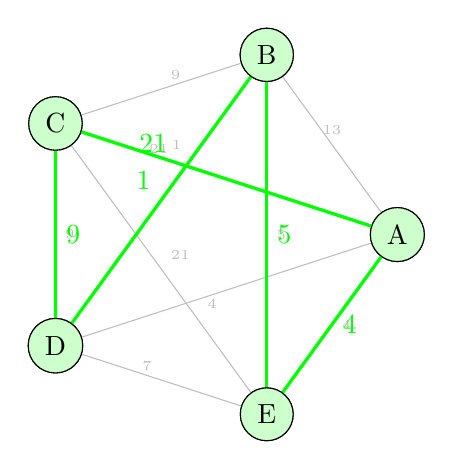
\begin{tikzpicture}[scale=0.8]
						% Define nodes
						\node[circle,draw,fill=green!20] (A) at (1 * 3,0) {A};
						\node[circle,draw] (B) at (0.309 * 3,0.951 * 3) {B};
						\node[circle,draw] (C) at (-0.809*3,0.588*3) {C};
						\node[circle,draw] (D) at (-0.809*3,-0.588*3) {D};
						\node[circle,draw] (E) at (0.309*3,-0.951*3) {E};

						% Draw all edges in light gray
						\ifthenelse{\step < 5}{%
							\draw[lightgray] (A) -- node[above] {\tiny 13} (B);
							\draw[lightgray] (A) -- node[below left] {\tiny 4} (D);
							\draw[lightgray] (A) -- node[pos = 2/3, above left] {\tiny 21} (C);
							\ifthenelse{\step < 1}{\draw[lightgray] (A) -- node[right] {\tiny 4} (E);}{}
							\draw[lightgray] (B) -- node[above right] {\tiny 9} (C);
							\ifthenelse{\step < 2}{\draw[lightgray] (B) -- node[right] {\tiny 5} (E);}{}

							\ifthenelse{\step < 4}{
								\draw[lightgray] (C) -- node[above right] {\tiny 21} (E);
								\draw[lightgray] (C) -- node[right] {\tiny 9} (D);}{}
							\draw[lightgray] (D) -- node[pos = 1/2, above left] {\tiny 7} (E);
							\ifthenelse{\step < 3}{\draw[lightgray] (B) -- node[pos = 1/3, above left] {\tiny 1} (D);}{}
						}{}

						% Highlight the path based on the step
						\ifthenelse{\step > 0}{%
							\draw[green,very thick] (A) -- node[right] {4} (E);
							\node[circle,fill=green!20,draw] at (A) {A};
						}{}
						\ifthenelse{\step > 1}{%
							\draw[green,very thick] (E) -- node[right] {5} (B);
							\node[circle,fill=green!20,draw] at (E) {E};
						}{}
						\ifthenelse{\step > 2}{%
							\draw[green,very thick] (B) -- node[above left] {1} (D);
							\node[circle,fill=green!20,draw] at (B) {B};
						}{}
						\ifthenelse{\step > 3}{%
							\draw[green,very thick] (D) -- node[right] {9} (C);
							\node[circle,fill=green!20,draw] at (D) {D};
						}{}
						\ifthenelse{\step > 4}{%
							\draw[green,very thick] (C) -- node[pos = 1/3, above left] {21} (A);
							\node[circle,fill=green!20,draw] at (C) {C};
						}{}
					\end{tikzpicture}
					\caption{Iterazione \step}
				\end{subfigure}%
				\ifnum\step>0
					\ifnum\numexpr\step+1\relax=3\relax
						\par\vspace{\baselineskip}
					\fi
				\fi
			}%
	\end{figure}
}


\tspnearestneighbor{6}

\paragraph{Pseudocode}

\begin{algorithm}
	\caption{TSP \Gls{NNS}}\label{alg:greedybestfirst}
	\begin{algorithmic}[1]
		\Procedure{NearestNeighborSearch}{$cities, distances$}
		\State $start \gets$ select an arbitrary city from $cities$
		\State $current \gets start$
		\State $tour \gets$ list containing $start$
		\State $unvisited \gets cities \setminus \{start\}$
		\While{$unvisited \neq \emptyset$}
		\State $next \gets$ city in $unvisited$ with minimum distance from $current$
		\State add $next$ to $tour$
		\State remove $next$ from $unvisited$
		\State $current \gets next$
		\EndWhile
		\State add $start$ to $tour$ to close the cycle
		\State \Return $tour$
		\EndProcedure
	\end{algorithmic}
\end{algorithm}

This greedy strategy ensures that at each step, the tour grows by adding the nearest possible destination, optimizing for the immediate next step without considering the overall tour length. While this method does not guarantee finding the shortest possible tour, it significantly reduces computation time compared to exhaustive search methods.

% TODO: Riordina questo

\subsubsection{Advantages and Limitations}

\textbf{Advantages:}
\begin{itemize}
	\item \textit{Simplicity}: Greedy algorithms are simple to implement and understand.
	\item \textit{Efficiency}: They often provide solutions quickly, making them suitable for problems where speed is crucial.
\end{itemize}

\textbf{Limitations:}
\begin{itemize}
	\item \textit{Optimality}: Greedy choices do not always lead to the optimal solution, especially for complex problems like the \Gls{TSP}.
	\item \textit{Short-sightedness}: By focusing on local optimality, they might overlook better solutions that require initially non-optimal choices.
\end{itemize}

Greedy algorithms, with their inherent simplicity and efficiency, play a crucial role in the heuristic resolution of problems, especially in cases where obtaining an exact solution is computationally impractical. Their application to the \Gls{TSP} highlights the balance between computational efficiency and solution quality, a theme that resonates through the study of heuristic and metaheuristic algorithms.


\begin{table}
	\centering
	\caption{Results of the Nearest Neighbor algorithm}
	\begin{tabular}{lrrrr}
		\toprule
		Instance  & Time (ms) & Tour Length & Optimal Length & Gap   \\
		\midrule
		berlin52 & 14         & 8980.92        & 7542.00          & 19.08 \\
		eil51    & 15         & 513.61         & 426.00           & 20.57 \\
		eil76    & 17         & 711.99         & 538.00           & 32.34 \\
		lin105   & 43         & 20362.76       & 14379.00         & 41.61 \\
		pr124    & 136        & 69299.43       & 59030.00         & 17.40 \\
		d198     & 183        & 18620.07       & 15780.00         & 18.00 \\
		lin318   & 466        & 54033.58       & 42029.00         & 28.56 \\
		u574     & 1295       & 46881.87       & 36905.00         & 27.03 \\
		fl1577   & 9547       & 27940.91       & 22249.00         & 25.58 \\
		rl5915   & 236473     & 707498.63      & 565530.00        & 25.10 \\
		\bottomrule
	\end{tabular}
\end{table}


\section{Local Search Algorithms}

Local search algorithms represent a class of heuristic methods designed to explore the solution space of an optimization problem by iteratively moving from one solution to a neighboring solution in the search space. These algorithms are particularly effective for problems such as the \Gls{TSP}. Local search provides a mechanism to improve an initial solution through small localized modifications \cite{Johnson2002,Lawler1985}.

\subsection{2-opt and 3-opt Techniques}

The 2-opt and 3-opt techniques are specific local search strategies used to refine \Gls{TSP} solutions. They work by iteratively removing two or three edges from the tour and reconnecting the segments in a different order, aiming to reduce the total tour length with each operation.

\subsubsection{2-opt Technique}

The 2-opt algorithm systematically checks each pair of edges in the tour and determines whether swapping them would lead to a shorter path. This process is repeated until no further improvements can be made.


\begin{center}
	\begin{figure}[h]
		\caption{2-opt swap}
		\begin{tikzpicture}
			% Definisci i nodi
			\node[draw=none, fill=none] (A) at (0,2) {A};
			\node[draw=none] (B) at (2,1.7) {B};
			\node[draw=none] (C) at (4,1.5) {C};
			\node[draw=none] (D) at (6,2) {D};

			\node[draw=none] (G) at (0,0) {G};
			\node[draw=none] (F) at (2,0.2) {F};
			\node[draw=none] (E) at (4,0.5) {E};

			% Collega i nodi
			\draw (A) -- (B);
			\draw[red] (B) -- (E);
			\draw (E) -- (D);
			\draw (D) -- (C);
			\draw[red] (C) -- (F);
			\draw (F) -- (G);
			\draw (G) -- (A);

			% Definisci i nodi
			\node[draw=none] (A2) at (10-2,2) {A};
			\node[draw=none] (B2) at (12-2,1.7) {B};
			\node[draw=none] (C2) at (14-2,1.5) {C};
			\node[draw=none] (D2) at (16-2,2) {D};

			\node[draw=none] (G2) at (10-2,0) {G};
			\node[draw=none] (F2) at (12-2,0.2) {F};
			\node[draw=none] (E2) at (14-2,0.5) {E};

			% Collega i nodi
			\draw (A2) -- (B2);
			\draw[blue] (B2) -- (C2);
			\draw (E2) -- (D2);
			\draw (D2) -- (C2);
			\draw[blue] (E2) -- (F2);
			\draw (F2) -- (G2);
			\draw (G2) -- (A2);
		\end{tikzpicture}
	\end{figure}
\end{center}

\begin{algorithm}
	\caption{2-opt Technique for \Gls{TSP}}\label{alg:twoopt}
	\begin{algorithmic}[1]
		\Procedure{TwoOpt}{$tour, distances$}
		\State $improved \gets true$
		\While{$improved$}
		\State $improved \gets false$
		\For{$i \gets 1$ to length($tour$) - 1}
		\For{$j \gets i+1$ to length($tour$)}
		\If{\Call{TwoOptSwap}{$tour, i, j$} $<$ \Call{TourDistance}{$tour$}}
		\State $tour \gets$ \Call{TwoOptSwap}{$tour, i, j$}
		\State $improved \gets true$
		\EndIf
		\EndFor
		\EndFor
		\EndWhile
		\State \Return $tour$
		\EndProcedure
	\end{algorithmic}
\end{algorithm}


\begin{table}
	\centering
	\caption{Results of Nearest Neighbor algorithm with 2-opt optimization}
	\begin{tabular}{lrrrr}
		\toprule
		Instance  & Time (ms) & Tour Length & Optimal Length & Gap   \\
		\midrule
		berlin52 & 124        & 8060.65        & 7542.00          & 6.88  \\
		eil51    & 284        & 440.90         & 426.00           & 3.50  \\
		eil76    & 313        & 599.05         & 538.00           & 11.35 \\
		lin105   & 2959       & 16199.70       & 14379.00         & 12.66 \\
		pr124    & 3268       & 62757.01       & 59030.00         & 6.31  \\
		d198     & 4443       & 16165.31       & 15780.00         & 2.44  \\
		lin318   & 9562       & 46408.41       & 42029.00         & 10.42 \\
		u574     & 26923      & 39896.00       & 36905.00         & 8.10  \\
		fl1577   & 200151     & 24214.30       & 22249.00         & 8.83  \\
		rl5915   & 6327036    & 620822.08      & 565530.00        & 9.78  \\
		\bottomrule
	\end{tabular}
\end{table}


\subsubsection{3-opt Technique}

The 3-opt technique extends the idea of 2-opt by considering three edges for reconnection. This allows a wider range of rearrangements at each step, potentially leading to more significant improvements at the cost of greater computational complexity.

\paragraph{Pseudocode for the 3-opt Technique} is conceptually similar to 2-opt but involves more conditions for swaps, reflecting the greater complexity of considering three edges at a time.

\subsection{Lin–Kernighan}

The Lin-Kernighan algorithm (\Gls{LK}) is one of the most advanced and powerful local search techniques for solving the \Gls{TSP}. Proposed by Shen Lin and Brian W. Kernighan in 1973, this algorithm extends the ideas of the \(k\)-opt technique, making it more flexible and adaptable. The algorithm is not limited to a fixed size \(k\) of swaps, but dynamically decides the number of edges to remove and reconnect, making it very effective in improving initial solutions.\cite{lin1973effective}


\begin{algorithm}
	\caption{Lin-Kernighan Algorithm for the \Gls{TSP}}\label{alg:lin-kernighan}
	\begin{algorithmic}[1]
		\Procedure{LinKernighan}{$T$} \Comment{$T$ is the initial tour}
		\State $T' \gets T$ \Comment{Initialize $T'$ with $T$}
		\Repeat
		\For{each city $x_1$ in $T'$}
		\State $k \gets 2$
		\Repeat
		\State Select a set of $k$ edges $(x_1, y_1), (x_2, y_2), \ldots, (x_k, y_k)$ from $T'$
		\State Generate a new tour $T''$ by removing edges and reconnecting according to the $k$-opt move
		\If{$T''$ is shorter than $T'$}
		\State $T' \gets T''$
		\State \textbf{break} \Comment{Exit inner loop if there is improvement}
		\EndIf
		\State $k \gets k + 1$
		\Until{No further improvement}
		\EndFor
		\Until{All cities have been tried as starting cities}
		\State \Return $T'$
		\EndProcedure
	\end{algorithmic}
\end{algorithm}
\subsubsection{Description}

The \Gls{LK} algorithm starts with an initial solution and attempts to iteratively improve this solution through a series of generalized \(k\)-opt moves. Each \(k\)-opt move seeks to reduce the total tour length by exchanging \(k\) edges of the current tour with new edges, thus improving the overall path.


The \Gls{LK} algorithm has been extensively studied and improved over the years. For a detailed analysis of the algorithm and its extensions, the following references can be consulted \cite{Johnson2002,Lawler1985,Gutin2016}.
\\

Local search algorithms, including 2-opt and 3-opt techniques, offer powerful methods for improving \Gls{TSP} solutions. By iteratively refining an initial solution, they balance exploration of the solution space and exploitation of known good configurations, providing effective means to approach optimal solutions for complex optimization problems.


\section{Metaheuristic Algorithms}

Metaheuristic algorithms are high-level strategies designed to navigate the search space of complex optimization problems efficiently. These algorithms do not guarantee an optimal solution, but are effective in finding very good solutions within a reasonable time frame, especially for problems where traditional methods fail due to the curse of dimensionality or the presence of numerous local optima.

\subsection{Simulated Annealing}

Simulated Annealing (\Gls{SA}) presents itself as a stochastic technique designed to approximate the global optimum of a given objective function. This method finds its roots in the physical process of annealing in metallurgy, which involves controlled heating and cooling of a material to increase the size of its crystals and reduce their defects. The SA algorithm mimics this process by introducing a metaphorical "temperature" that gradually decreases according to a predetermined schedule. Initially, the algorithm is more inclined to accept solutions that are worse than the current solution, allowing it to explore the solution space widely and avoid becoming trapped in local optima prematurely. As the temperature decreases, the algorithm becomes more selective, focusing on the optimal solution.

\subsubsection{Application to the \Gls{TSP}}

In the context of the \Gls{TSP}, the SA algorithm starts with an arbitrary solution, typically a random tour among the cities. Subsequently, it iteratively refines this tour by making slight modifications, such as swapping two cities in the tour sequence. The decision to accept a new solution is probabilistic and depends on both the difference in solution quality and the current temperature. This method's ability to accept worse solutions decreases probabilistically over time as the temperature lowers, simulating the cooling process in annealing.


\begin{table}[H]
  \centering
	\caption{Results of the Simulated Annealing algorithm}
	\begin{tabular}{lrrrr}
		\toprule
		Instance  & Time (ms) & Tour Length & Optimal Length & Gap   \\
		\midrule
		berlin52 & 28982      & 7544.37        & 7542.00          & 0.03  \\
		87eil76  & 39587      & 572.81         & 538.00           & 6.47  \\
		29lin105 & 52928      & 14993.92       & 14379.00         & 4.28  \\
		44d198   & 102362     & 16318.76       & 15780.00         & 3.41  \\
		49eil51  & 131542     & 434.25         & 426.00           & 1.94  \\
		pr124    & 207125     & 60675.98       & 59030.00         & 2.79  \\
		67u574   & 398181     & 43936.09       & 36905.00         & 19.05 \\
		lin318   & 506369     & 47651.44       & 42029.00         & 13.38 \\
		fl1577   & 1514830    & 27584.16       & 22249.00         & 23.98 \\
		rl5915   & 22563370   & 680777.61      & 565530.00        & 20.38 \\
		\bottomrule
	\end{tabular}
\end{table}

\paragraph{Pseudocode}

The pseudocode for applying \Gls{SA} to solve the \Gls{TSP} is outlined below. This algorithmic representation emphasizes the iterative improvement of a tour, taking into account the acceptance of suboptimal solutions based on a decreasing temperature schedule to escape local minima.

\begin{algorithm}
	\caption{Simulated Annealing}\label{alg:detailedsimulatedannealing}
	\begin{algorithmic}[1]
		\Procedure{SATSP}{$cities, initialTemp, coolingRate, stoppingTemp$}
		\State $bestSolution \gets generateInitialSolution(cities)$
		\State $currentSolution \gets bestSolution$
		\State $currentTemp \gets initialTemp$
		\While{$currentTemp > stoppingTemp$}
		\State $newSolution \gets$ perturbSolution($currentSolution, cities$)
		\State $currentCost \gets$ calculateCost($currentSolution$)
		\State $newCost \gets$ calculateCost($newSolution$)
		\State $acceptanceProb \gets$ AcceptanceProbability($currentCost, newCost, currentTemp$)
		\If{acceptanceProb $>$ randomValue(0, 1)}
		\State $currentSolution \gets newSolution$
		\If{newCost < calculateCost($bestSolution$)}
		\State $bestSolution \gets newSolution$
		\EndIf
		\EndIf
		\State $currentTemp \gets$ updateTemperature($currentTemp, coolingRate$)
		\EndWhile
		\State \textbf{return} $bestSolution$
		\EndProcedure
	\end{algorithmic}
\end{algorithm}

In this pseudocode, \emph{generateInitialSolution} creates a random initial tour of the cities. \emph{perturbSolution} slightly alters the current solution, typically by swapping two cities in the tour. \emph{calculateCost} evaluates the total distance (or cost) of a tour. \emph{calculateAcceptanceProbability} determines the probability of accepting a new solution based on its cost, the cost of the current solution, and the current temperature, following the Metropolis criterion\cite{metropolis1953equation}. The temperature is updated in each iteration by the \emph{updateTemperature} function, which reduces the temperature based on the cooling rate until reaching the stopping temperature.

\subsection{Genetic Algorithms}

Genetic Algorithms (\Gls{GA}) are a class of heuristic methods inspired by the principles of biological evolution and natural selection. Introduced by John Holland in the 1960s, these algorithms are particularly effective in tackling complex and nonlinear optimization problems, such as the \Gls{TSP}.

\subsubsection{Fundamental Principles}

Genetic algorithms operate on a population of potential solutions, encoded as "chromosomes". The fundamental principles include:

\begin{itemize}
	\item \textbf{Selection}: The best (most "fit") solutions are more likely to be selected for reproduction.
	\item \textbf{Crossover}: Combination of parts from two parent solutions to create a new one.
	\item \textbf{Mutation}: Random modifications introduced in solutions to maintain genetic diversity.
	\item \textbf{Evolution}: New generations tend to improve over time, converging toward optimal or near-optimal solutions.
\end{itemize}

\subsubsection{Application to the \Gls{TSP}}

In the context of the \Gls{TSP}, a genetic algorithm typically operates as follows:

\begin{enumerate}
	\item \textbf{Encoding}: Each tour is represented as a sequence of cities (chromosome).
	\item \textbf{Initial population}: Generation of a random set of valid tours.
	\item \textbf{Fitness function}: Evaluation of the length of each tour (fitness inversely proportional to length).
	\item \textbf{Selection}: Choice of the best tours for reproduction (e.g., tournament or roulette selection).
	\item \textbf{Crossover}: Combination of parts from two parent tours (e.g., partially mapped crossover - PMX).
	\item \textbf{Mutation}: Small random modifications in tours (e.g., swapping two cities).
	\item \textbf{Replacement}: Creation of a new generation by combining parents and offspring.
	\item \textbf{Iteration}: Repetition of the process for a fixed number of generations or until reaching a stopping criterion.
\end{enumerate}
\begin{table}[H]
	\centering
	\caption{Results of the Genetic Algorithm}
	\begin{tabular}{lrrrr}
		\toprule
		Instance  & Time (ms) & Tour Length & Optimal Length & Gap   \\
		\midrule
		eil51    & 22815      & 440.85         & 426.00           & 3.49  \\
		berlin52 & 26104      & 7918.09        & 7542.00          & 4.99  \\
		eil76    & 44547      & 570.63         & 538.00           & 6.06  \\
		d198     & 108498     & 16548.42       & 15780.00         & 4.87  \\
		lin105   & 109871     & 14573.34       & 14379.00         & 1.35  \\
		pr124    & 137120     & 61453.95       & 59030.00         & 4.11  \\
		lin318   & 320190     & 45165.59       & 42029.00         & 7.46  \\
		u574     & 1260895    & 40516.22       & 36905.00         & 9.79  \\
		fl1577   & 4033113    & 24024.81       & 22249.00         & 7.98  \\
		rl5915   & 33367821   & 648205.16      & 565530.00        & 14.62 \\
		\bottomrule
	\end{tabular}
\end{table}

\subsubsection{Pseudocode}


\begin{algorithm}
	\caption{Genetic Algorithm for \Gls{TSP}}\label{alg:geneticalgorithm}
	\begin{algorithmic}[1]
		\Procedure{GeneticAlgorithmTSP}{$cities, populationSize, generations, mutationRate$}
		\State $population \gets$ InitializePopulation($cities, populationSize$)
		\For{$g \gets 1$ to $generations$}
		\State EvaluateFitness($population$)
		\State $newPopulation \gets \emptyset$
		\While{$|newPopulation| < populationSize$}
		\State $parent1 \gets$ SelectParent($population$)
		\State $parent2 \gets$ SelectParent($population$)
		\State $child \gets$ Crossover($parent1, parent2$)
		\If{Random() $< mutationRate$}
		\State Mutate($child$)
		\EndIf
		\State $newPopulation \gets newPopulation \cup \{child\}$
		\EndWhile
		\State $population \gets newPopulation$
		\EndFor
		\State \Return BestSolution($population$)
		\EndProcedure
	\end{algorithmic}
\end{algorithm}

\subsubsection{Advantages}

Genetic algorithms offer several significant advantages for solving the \Gls{TSP}:

\begin{itemize}
	\item \textbf{Global exploration}: Ability to explore broad regions of the solution space, reducing the risk of premature convergence to local optima.
	\item \textbf{Parallelizability}: The population-based nature lends itself well to parallel computation, improving computational efficiency.
	\item \textbf{Flexibility}: Easily adaptable to variants of the \Gls{TSP} and other combinatorial optimization problems.
	\item \textbf{Robustness}: Ability to handle noisy or ill-defined objective functions.
	\item \textbf{Multiple solutions}: Can provide a set of good solutions, not just a single optimal solution.
\end{itemize}

\subsubsection{Disadvantages}

Despite their strengths, Genetic Algorithms also present some limitations:

\begin{itemize}
	\item \textbf{Convergence time}: May require many generations to converge, especially for large-scale problems.
	\item \textbf{Parameter sensitivity}: Performance depends heavily on the choice of parameters such as population size, mutation rate, selection method, etc.
	\item \textbf{No guarantee of global optimum}: Like other metaheuristics, they do not guarantee finding the global optimal solution.
	\item \textbf{Encoding difficulty}: For some problems, effective representation of solutions as "chromosomes" can be complex.
	\item \textbf{Loss of diversity}: May suffer from premature convergence if not properly managed, leading to sub-optimal solutions.
\end{itemize}

\subsubsection{Variants and Improvements}

Numerous variants and improvements have been proposed to optimize the performance of Genetic Algorithms for the \Gls{TSP}:

\begin{itemize}
	\item \textbf{Specialized crossover operators}: Such as \Gls{PMX} (Partially Mapped Crossover) or \Gls{OX} (Order Crossover), specifically designed to preserve the relative order of cities.
	\item \textbf{Diversification techniques}: Introduction of mechanisms to maintain population diversity, such as "crowding" or "ecological niching".
	\item \textbf{Hybridization}: Combination with local search techniques (such as 2-opt) for fine optimization of solutions.
	\item \textbf{Parameter adaptation}: Strategies to dynamically adjust algorithm parameters during execution.
	\item \textbf{Alternative representations}: Use of different encodings for tours, such as path-based or adjacency-based representation.
\end{itemize}


Genetic Algorithms represent a powerful and flexible approach to tackling the \Gls{TSP} and other combinatorial optimization problems. Their ability to effectively explore vast and complex solution spaces makes them particularly suitable for large-scale instances or those with non-standard characteristics. However, the effectiveness of Genetic Algorithms depends heavily on the appropriate choice of genetic operators, parameters, and implementation strategies. Ongoing research in this field aims to further improve the performance and applicability of these algorithms to an increasingly wide range of optimization problems.

\subsection{Tabu Search}

Tabu Search (\Gls{TS}) is an optimization metaheuristic that extends local search by incorporating memory structures to guide the search process. Introduced by Fred Glover in 1986, this technique is particularly effective for combinatorial optimization problems such as the \Gls{TSP}.

\subsubsection{Fundamental Principles}

The key idea of \Gls{TS} is the use of adaptive memory (the tabu list) to avoid returning to recently visited solutions, thus allowing the algorithm to explore new areas of the solution space and potentially escape local optima. The tabu list stores characteristics of recent solutions or moves made, temporarily prohibiting their reuse.

\subsubsection{Application to the \Gls{TSP}}

In the context of the \Gls{TSP}, Tabu Search typically operates as follows:

\begin{enumerate}
	\item Starts with an initial solution (a complete tour).
	\item At each iteration, explores the neighborhood of the current solution (e.g., by swapping pairs of cities).
	\item Selects the best non-tabu move, even if it worsens the current solution.
	\item Updates the tabu list, adding the move just made and removing older moves if necessary.
	\item Repeats the process for a predefined number of iterations or until a stopping criterion is met.
\end{enumerate}

\subsubsection{Pseudocode}


\begin{algorithm}
	\caption{Tabu Search for \Gls{TSP}}\label{alg:tabusearch}
	\begin{algorithmic}[1]
		\Procedure{TabuSearchTSP}{$initialSolution, maxIterations, tabuListSize$}
		\State $currentSolution \gets initialSolution$
		\State $bestSolution \gets currentSolution$
		\State $tabuList \gets$ initialize empty list
		\For{$iteration \gets 1$ to $maxIterations$}
		\State $neighborhood \gets$ generateNeighborhood($currentSolution$)
		\State $bestCandidate \gets$ null
		\For{$candidate$ in $neighborhood$}
		\If{($candidate$ better than $bestCandidate$ AND move not in $tabuList$) OR\\
			\qquad ($candidate$ better than $bestSolution$)}
		\State $bestCandidate \gets candidate$
		\EndIf
		\EndFor
		\State $currentSolution \gets bestCandidate$
		\If{$currentSolution$ better than $bestSolution$}
		\State $bestSolution \gets currentSolution$
		\EndIf
		\State Update $tabuList$
		\EndFor
		\State \Return $bestSolution$
		\EndProcedure
	\end{algorithmic}
\end{algorithm}

\subsubsection{Advantages}

\Gls{TS} offers several significant advantages:

\begin{itemize}
	\item \textbf{Avoids local optima}: The tabu list allows the algorithm to temporarily accept worsening moves, helping to escape local optima.
	\item \textbf{Efficient exploration}: Effectively balances exploration of new areas of the solution space and exploitation of found good solutions.
	\item \textbf{Adaptability}: Can be easily adapted to various combinatorial optimization problems.
	\item \textbf{Short and long-term memory}: Can incorporate short and long-term memory strategies to guide the search more intelligently.
\end{itemize}

\subsubsection{Disadvantages}

Despite its strengths, \Gls{TS} also presents some limitations:

\begin{itemize}
	\item \textbf{Parameter sensitivity}: Performance can depend heavily on the choice of parameters, such as the tabu list size and aspiration criteria.
	\item \textbf{Computational complexity}: Exploring the neighborhood at each iteration can be computationally expensive for large-scale problems.
	\item \textbf{No guarantee of global optimum}: Like other metaheuristics, it does not guarantee finding the global optimal solution.
	\item \textbf{Implementation difficulty}: Efficient implementation of memory structures and aspiration criteria can be complex.
\end{itemize}


\Gls{TS} represents a powerful tool in the arsenal of metaheuristics for the \Gls{TSP} and other combinatorial optimization problems. Its ability to avoid local optima and effectively explore the solution space makes it particularly suitable for large-scale or complex problem instances. However, like many advanced techniques, its effectiveness depends on careful calibration and implementation.

\section{Ant Colony Optimization}

Ant Colony Optimization (\Gls{ACO}) is a metaheuristic algorithm inspired by the behavior of real ant colonies \cite{dorigo1996ant}. This approach simulates the way ants find the shortest paths between food sources and their nest, applying this concept to solving combinatorial optimization problems such as the \Gls{TSP} \cite{dorigo1997ant}.

\subsection{Fundamental Principles of \Gls{ACO}}

\Gls{ACO} is based on several key principles:

\begin{enumerate}
	\item \textbf{Pheromones}: Ants deposit a chemical substance called pheromone along the paths they follow. This serves as an indirect communication mechanism among ants \cite{dorigo2006ant}.
	\item \textbf{Evaporation}: Pheromones evaporate over time, allowing the algorithm to "forget" less optimal paths and prevent premature convergence \cite{stutzle2000max}.
	\item \textbf{Choice probability}: Ants choose their path based on the amount of pheromones present and the distance between cities, with an element of randomness \cite{dorigo2004ant}.
\end{enumerate}

\subsection{Application to the \Gls{TSP}}

In the context of the \Gls{TSP}, ACO operates as follows:

\begin{enumerate}
	\item \textbf{Initialization}: A small amount of pheromones is deposited on all possible paths.
	\item \textbf{Tour Construction}: Each ant constructs a complete tour, choosing the next city to visit based on the formula:

	      \[P_{ij}^k = \frac{(\tau_{ij})^\alpha \cdot (\eta_{ij})^\beta}{\sum_{l \in N_i^k} (\tau_{il})^\alpha \cdot (\eta_{il})^\beta}\]

	      where:
	      \begin{itemize}
		      \item $P_{ij}^k$ is the probability that ant $k$ moves from city $i$ to city $j$
		      \item $\tau_{ij}$ is the amount of pheromone on path $(i,j)$
		      \item $\eta_{ij}$ is the inverse of the distance between cities $i$ and $j$
		      \item $\alpha$ and $\beta$ are parameters that control the relative importance of pheromones and distance
		      \item $N_i^k$ is the set of cities not yet visited by ant $k$
	      \end{itemize}

	\item \textbf{Pheromone Update}: After all ants have completed their tours, pheromones are updated according to the formula:

	      \[\tau_{ij} = (1-\rho)\tau_{ij} + \sum_{k=1}^m \Delta\tau_{ij}^k\]

	      where:
	      \begin{itemize}
		      \item $\rho$ is the pheromone evaporation rate
		      \item $m$ is the number of ants
		      \item $\Delta\tau_{ij}^k$ is the amount of pheromone deposited by ant $k$ on path $(i,j)$, usually proportional to the quality of the tour found
	      \end{itemize}

	\item \textbf{Iteration}: Steps 2 and 3 are repeated for a predefined number of iterations or until a termination criterion is reached.
\end{enumerate}

The following pseudocode describes the basic implementation of \Gls{ACO} for the \Gls{TSP}:

\begin{algorithm}
	\begin{algorithmic}[1]
		\Procedure{ConstructTour}{$G, \alpha, \beta$}
		\State Choose a random starting city
		\While{there are unvisited cities}
		\State Choose the next city using the probability formula
		\EndWhile
		\State \Return complete tour
		\EndProcedure

		\Procedure{UpdatePheromones}{$G, \rho, Q$}
		\For{each edge $(i,j)$ in $G$}
		\State $\tau_{ij} \gets (1-\rho)\tau_{ij}$
		\For{$k = 1$ to $m$}
		\If{$(i,j)$ is in $tour_k$}
		\State $\tau_{ij} \gets \tau_{ij} + Q/length_k$
		\EndIf
		\EndFor
		\EndFor
		\EndProcedure
	\end{algorithmic}
\end{algorithm}

\begin{algorithm}
	\caption{\Gls{ACO} for the \Gls{TSP}}\label{alg:aco-tsp}
	\begin{algorithmic}[1]
		\Procedure{ACO-TSP}{$G, m, \alpha, \beta, \rho, Q, max\_iterations$}
		\State $G \gets$ graph of cities
		\State $m \gets$ number of ants
		\State $\alpha, \beta \gets$ control parameters
		\State $\rho \gets$ pheromone evaporation rate
		\State $Q \gets$ constant for pheromone deposit
		\State $max\_iterations \gets$ maximum number of iterations

		\State Initialize pheromones $\tau_{ij} = \tau_0$ for each edge $(i,j)$ in $G$
		\State $best\_tour \gets \emptyset$
		\State $best\_length \gets \infty$

		\For{$iteration = 1$ to $max\_iterations$}
		\For{$k = 1$ to $m$}
		\State $tour_k \gets$ ConstructTour($G, \alpha, \beta$)
		\State $length_k \gets$ CalculateTourLength($tour_k$)
		\If{$length_k < best\_length$}
		\State $best\_tour \gets tour_k$
		\State $best\_length \gets length_k$
		\EndIf
		\EndFor

		\State UpdatePheromones($G, \rho, Q$)
		\EndFor

		\State \Return $best\_tour, best\_length$
		\EndProcedure

	\end{algorithmic}
\end{algorithm}

The procedures \texttt{ConstructTour} and \texttt{UpdatePheromones} are represented in simplified form and can be further detailed in an actual implementation.

\subsection{Variants and Improvements}

Several variants of \Gls{ACO} have been proposed to improve algorithm performance on the \Gls{TSP}:

\begin{itemize}
	\item \textbf{MAX-MIN Ant System (\Gls{MMAS})}: Introduces upper and lower limits to the amount of pheromones, preventing stagnation \cite{stutzle2000max}.
	\item \textbf{Ant Colony System (\Gls{ACS})}: Uses a more aggressive transition rule and local pheromone update \cite{dorigo1997ant}.
	\item \textbf{Rank-Based Ant System}: Modifies the pheromone update rule based on the quality of tours found \cite{bullnheimer1999rank}.
\end{itemize}

\subsection{Advantages and Challenges}

ACO offers several advantages for solving the \Gls{TSP}:

\begin{itemize}
	\item \textbf{Adaptability}: Can easily adapt to changes in the problem, such as adding or removing cities.
	\item \textbf{Solution quality}: Often finds high-quality solutions, especially for large-scale \Gls{TSP} instances.
\end{itemize}

However, \Gls{ACO} also presents some challenges:

\begin{itemize}
	\item \textbf{Convergence}: May converge prematurely to sub-optimal solutions if parameters are not correctly calibrated.
	\item \textbf{Computation time}: For large-scale problems, may require significant computation time to reach high-quality solutions.
	\item \textbf{Parameterization}: Algorithm effectiveness depends heavily on parameter choice, which can be difficult to optimize.
\end{itemize}

\subsection{Conclusions}

\Gls{ACO} represents a powerful and flexible approach to tackling the Traveling Salesman Problem. Drawing inspiration from the natural foraging processes of ants, \Gls{ACO} offers a robust mechanism for exploring the solution space of the \Gls{TSP}, effectively balancing the exploration of new solutions with the exploitation of accumulated information. Despite challenges related to parameterization and computation time, \Gls{ACS} continues to be an active area of research and development in the field of combinatorial optimization \cite{dorigo2010ant}.
